\documentclass{article}
% common packages used in maths
\usepackage{amsmath}
\usepackage{amsthm}%possible problem
\usepackage{amssymb}
\usepackage{amsfonts}
% for including figures with \includegraphics{}
\usepackage{graphicx}
\author{
Pascal Zürcher 22-111-314 & 
Leandro Lüthi 22-105-035 & 
Manuel Flückiger 22-112-502}
\title{Lineare Algebra Serie 6 Übungsaufgaben}
\date{\today}

\begin{document}
\maketitle
\section{Finden Sie fur die folgenden Vektorräume jeweils eine Basis und
bestimmen Sie die Dimension des Vektorraums (Begründen Sie Ihre Antworten!):}
    \begin{enumerate}

        \item[a)] \[\{(x_1, x_2, x_3, x_4) ∈ \mathbb{R}^4   : x_1 = 2x_2, x_1 + x_4 = x_3\}\]
        Da $x_1 = 2x_2$ sind $x_1$ und $x_2$ linear 
        unabhängig. da $x_1 + x_4 = x_3$ gilt, ist $x_3$ von $x_1$ und $x_4$ 
        abhängig. Somit sind nur $x_1$ und $x_4$ linear unabhängig.
        Damit ist dim = 2 und eine mögliche Basis ist:
        \[<x_1, x_4> ,
        <\left(\begin{array}{c}2\\1\\2\\0\end{array}\right),
        \left(\begin{array}{c}2\\1\\3\\1\end{array}\right)>\]

        \item[b)]\[\{(x_1, x_2, x_3, x_4) ∈ \mathbb{R}^4   : x_1+3x_2+x_3+2x_4=0\}\]
        \newline
        $\alpha x_1 + \beta x_2 + \gamma x_3 + \delta x_4 = 0$ wenn $\alpha = \beta=\delta=0$
        gelten müsste, um diese Gleichung zu erfüllen, wären $x_1,x_2,x_3,x_4$ linear unabhängig.
        Daraus folgt, dass nicht alle linear unabhängig sind. $x_1+3x_2+x_3+2x_4 = 0$ Da es zur 
        Darstellung einer der Vektoren immer alle drei Anderen benötigt (siehe (*)), sind 
        drei Vektoren linear unabhängig. Somit ist dim = 3 und eine mögliche Basis 
        ist: 
        \[basis <x_1,x_3,x_4>\]
        \fbox{\parbox{\linewidth}{
        \begin{itemize}
            \item[] $x_1 = -3x_2-x_3-2x_4$
            \item[] $x_2 = -\frac{1}{5}x_1-x_3-\frac{2}{3}x_4$
            \item[] $x_3 = -x_1-3x_2-2x_4$
            \item[] $x_4 = -\frac{1}{2}x_1-\frac{3}{2}x_2-\frac{1}{2}x_3$
        \end{itemize}}}

        \item[c)] \[Mat(2,2;\mathbb{R})\]
        \newline
        $Mat(2,3,\mathbb{R})$ ist isomorph zu $\mathbb{R}^6$, da jedes 
        Elemente der Matrix irgend ein Element aus $\mathbb{R}$ ist.
        Somit ist dim = 6 und eine Basis zum Beispiel:
        \[basis\left<
        \left(\begin{array}{cc}1&0\\0&0\\0&0\end{array}\right),
        \left(\begin{array}{cc}0&0\\1&0\\0&0\end{array}\right),
        \left(\begin{array}{cc}0&0\\0&0\\1&0\end{array}\right),
        \left(\begin{array}{cc}0&1\\0&0\\0&0\end{array}\right),
        \left(\begin{array}{cc}0&0\\0&1\\0&0\end{array}\right),
        \left(\begin{array}{cc}0&0\\0&0\\0&1\end{array}\right),\right>\]

        \item[d)]\[\left\{\left(\begin{array}{cc}\alpha&\beta\\\beta&\gamma\end{array}\right)
        :\alpha,\beta,\gamma\in\mathbb{R}\right\}\subseteq Mat(2,2;\mathbb{R})\]
        \newline
        $a_{12}$ und $a_{21}$ müssen den gleichen Wert haben, also:
        \newline
        \[\alpha\left(\begin{array}{cc}1&0\\0&0\end{array}\right)+
        \beta\left(\begin{array}{cc}0&1\\1&0\end{array}\right)+
        \gamma\left(\begin{array}{cc}0&0\\0&1\end{array}\right)\]
        \newline
        Die drei Matrizen bilden die Basis mit drei Variablen $\Rightarrow$ dim = 3. Eine mögliche Basis ist:
        \[basis\left<\left(\begin{array}{cc}1&0\\0&0\end{array}\right),
        \left(\begin{array}{cc}0&1\\1&0\end{array}\right),
        \left(\begin{array}{cc}0&0\\0&1\end{array}\right)\right>\]

        \item[e)]\[Span\{1+x, x+x^2, x^2+x^3,1+x^2,x+x^3\}\subseteq Pol \mathbb{R}\]
        \newline
        U=Span\[\left\{
            \left(\begin{array}{c}1\\1\\0\\0\end{array}\right)
            \left(\begin{array}{c}0\\1\\1\\0\end{array}\right)
            \left(\begin{array}{c}0\\0\\1\\1\end{array}\right)
            \left(\begin{array}{c}1\\0\\1\\0\end{array}\right)
            \left(\begin{array}{c}0\\1\\0\\1\end{array}\right)
        \right\}\]
        \[
        \left( \begin{array}{ccccccc}
            1&0&0&1&0&|&0\\
            1&1&0&0&1&|&0\\
            0&1&1&1&0&|&0\\
            0&0&1&0&1&|&0\\
        \end{array}\right)
        \rightarrow
        \left( \begin{array}{ccccccc}
            1&0&0&1&0&|&0\\
            0&1&0&-1&1&|&0\\
            0&1&1&1&0&|&0\\
            0&0&1&0&1&|&0\\
        \end{array}\right)
        \]
        \[
        \rightarrow
        \left( \begin{array}{ccccccc}
            1&0&0&1&0&|&0\\
            0&1&0&-1&1&|&0\\
            0&0&1&2&-1&|&0\\
            0&0&1&0&1&|&0\\
        \end{array}\right)
        \rightarrow
        \left( \begin{array}{ccccccc}
            1&0&0&1&0&|&0\\
            0&1&0&-1&1&|&0\\
            0&0&1&2&-1&|&0\\
            0&0&0&-2&0&|&0\\
        \end{array}\right)
        \]\[
        \rightarrow
        \left( \begin{array}{ccccccc}
            1&0&0&0&1&|&0\\
            0&1&0&0&1&|&0\\
            0&0&1&0&-1&|&0\\
            0&0&0&-2&0&|&0\\
        \end{array}\right)\]
        
        dim = 4, da vier Pivot-Vektoren existieren und eine 
        Basis ist: 
        \[basis<(1),(x),(x^2),(-2x^3),(die Pivot-Vektoren)\]

        \item[f)]\[\{p(x)\in Pol_s \mathbb{R}: p(1)=0\}\]
        \[p(x)=a_0+a_1x+a_2x^2+a_3x^3\]
        \[p(1)=0\Rightarrow a_0=-a_1-a_2-a_3 (a_0+a_11+a_21^2+a_31^3=0)\]
        $\Rightarrow$\ Basis\ ist:
        \[\{(-1+x),(-x^2),(-1+x^3)\}:3\ Komponenten \Rightarrow dim = 3\]

        \item[g)]\[\{p(x)\in Pol_s \mathbb{R}: p(1)=p(-1)=0\}\]
        \[p(x)=ax^3+bx^2+cx+d\]
        \[p(1)=a+b+c+d=0\]
        \[p(-1)=-1+b-c+d=0\]
        \[a+b+c+d=-a+b-c+d |+a,+c,-b,-d\]
        \[2a+2c=0 |:2\]
        \[a+c=0 |-c\]
        \[a=-c\]
        \[\Rightarrow -c+b+c+d=c+b-c+d = 0\]
        \[b+d=b+d== |-d\]
        \[b=b=-d\]
        Wir schreiben die Polynome als Vektor ein in \{$x^3,x^2,x,1$\}
        \[
        \left(\begin{array}{c}a\\b\\c\\d\end{array}\right)=
        \left(\begin{array}{c}-c\\-d\\c\\d\end{array}\right)=
        \left(\begin{array}{c}-1\\0\\1\\0\end{array}\right)+d
        \left(\begin{array}{c}0\\-1\\0\\1\end{array}\right)
        \]
        $\left(\begin{array}{c}-1\\0\\1\\0\end{array}\right),\left(\begin{array}{c}0\\-1\\0\\1\end{array}\right)$, 
        sind linear unabhängig, da wenn $c\cdot 1=0$ oder \newline$c\cdot(-1)=0$, $c=0$ sein muss.
        Die Dimension beträgt dim = 2.
        eine Basis ist:
        \[<(x-x^3),(1-x^2)>\]

        \item[h)]\[f\in Abb(\mathbb{R},\mathbb{R}):f(x)=0\ bis\ auf\ endlich\ viele\ x\ \in \mathbb{R}\]
        Sei B eine endliche Basis von h). Jedes $b_o \in B$ hat endlich viele Inputwerte \neq 0.
        \[\Rightarrow\ Span\ B\ hat\ endlich\ viele\ Inputwerte\ \neq 0\]
        \[\Rightarrow h)\ hat\ keine\ endliche\ Basis\ dim\ (h)\ = \infty\]        
    \end{enumerate}

    \section{}
    \begin{enumerate}

        \item[a)]Sei V ein Vektorraum über K und seien $v_1,\dots,v_n$ linear unabhängig und 
        $v_{n+1}\in V$\textbackslash Span$\{v_1,\dots,v_n\}$. Zeigen Sie, dass $v_1,\dots,v_n,v_{n+1}$ 
        linear unabhängig sind
        \begin{enumerate}
            \item[Fall 1:]
            \[\lambda_{n+1}=0\]
            \Rightarrow\ widerspruch,\ da\ $v_1,\dots,v_n$\ linear\ unabhängig\ sind.
            \item[Fall 2:]
            \[\lambda_{n+1}\neq0\]
            \[\Rightarrow V_{n+1}=\frac{-\lambda_1}{\lambda_{n+1}}v_1-\dots-\frac{\lambda_n}{\lambda_{n+1}}v_n\]
            \Rightarrow\ widerspruch\ zu\ $v_{n+1} \notin Span\{v_1,\dots,v_n\}$.
        \end{enumerate}

        \item[b)]Seien V und W Vektorräume über K und sei $b_1,\dots,b_n$ eine Basis von W. Zeigen Sie, 
        dass für jede Abbildung $f:V \rightarrow W$ sind äquivalent:
        \begin{enumerate}
            \item[(i)] $f:V \rightarrow W$ ist ein Homomorphismus.
            \item[(ii)]Es gibt $f_1,\dots,f_n \in V^*$ mit $f(v)=f_1(v)b_1+\dots+f_n(v)b_n \forall v \in V$.
        \end{enumerate}
        "(ii)\Rightarrow (i)"
        \newline
        \[f(v)+f(u)=f_1(v)b_1+\dots+f_n(v)b_n+f_1(u)b_1+\dots+f_n(u)b_n\]
        \[=f_1(v)b_1+f_1(u)b_1+\dots+f_n(v)b_n+f_n(u)b_n\]
        \[=f_1(v+u)b_1+\dots+f_n(v+u)b_n\]
    \end{enumerate}

    \section{Sei V ein Vektorraum über K und $v_1,\dots,v_n\in V$. Betrachten Sie die folgenden Aussagen:}
    \begin{enumerate}
        \item[(i)] $_1v_1+\dots+a_nv_n=0$ hat nur die Lösung $a_1 = \dots = a_n = 0$
        \item[(ii)] Es existieren keine Koeffizienten $(\lambda_1,\dots,\lambda_{n-1})\neq(0,\dots,0)$, 
        so dass $v_n = \lambda_1v_1 + \dots+\lambda_{n-1}v_{n-1}$.
        \begin{proof} Wir beweisen das erste durch Kontraposition
            \begin{enumerate}
                \item["(i)$\Rightarrow$(ii)"]
                Es gibt einen $\lambda_1,\dots,\lambda_n \neq (0,\dots,0)$ und 
                $v_n=\lambda_1v_1+\lambda_2v_2+\dots+\lambda_{n-1}v_{n-1}$. Wir sehen, 
                dass $v_n$ per Definition eine Linearkombination ist. Daraus folgt, 
                dass $v_1,v_2,\dots,v_n$ linear abhängig sind.
                \item["(ii)$\nRightarrow$(i)"] Wir zeigen die Behauptung anhand eines Gegenbeispiels.
                \newline
                Seien $v_1=\left(\begin{array}{c}1\\0\\2\end{array}\right), v_2=\left(\begin{array}{c}2\\0\\4\end{array}\right)$ und 
                $v_3=\left(\begin{array}{c}0\\0\\1\end{array}\right)$.
                \newline
                Nun gibt es keine Koeffizienten $\lambda_1,\lambda_2$, beide ungleich Null, so dass gilt:
                \[v_3 = \lambda_1v_1+\lambda_2v_2 \ und\ \left(\begin{array}{c}0\\0\\1\end{array}\right) = 
                \lambda_1\left(\begin{array}{c}1\\0\\2\end{array}\right)+
                \lambda_2\left(\begin{array}{c}2\\0\\5\end{array}\right)\]
                Jedoch sind $v_1, v_2$ und $v_3$ trivialerweise linear abhängig.
            \end{enumerate}
        \end{proof}
    \end{enumerate}

    \section{}
    \begin{enumerate}
        \item[a)] Seien $U$, $W$ Unterräume eines endlich-dimensionalen Vektorraums $V$ über $K$ 
        mit dim $U$ + dim $W$ > dim $V$ . Zeigen Sie, dass $U \cap W \neq \{0\}$.

        \item[b)] Sei $V$ ein endlich-dimensionaler Vektorraum über $K$ und sei $A \cup \{a\} \subseteq V$.
        Zeigen Sie, dass \[a \in Span\ A \Leftrightarrow Rang\ A =\ Rang A \cup \{a\}.\]
        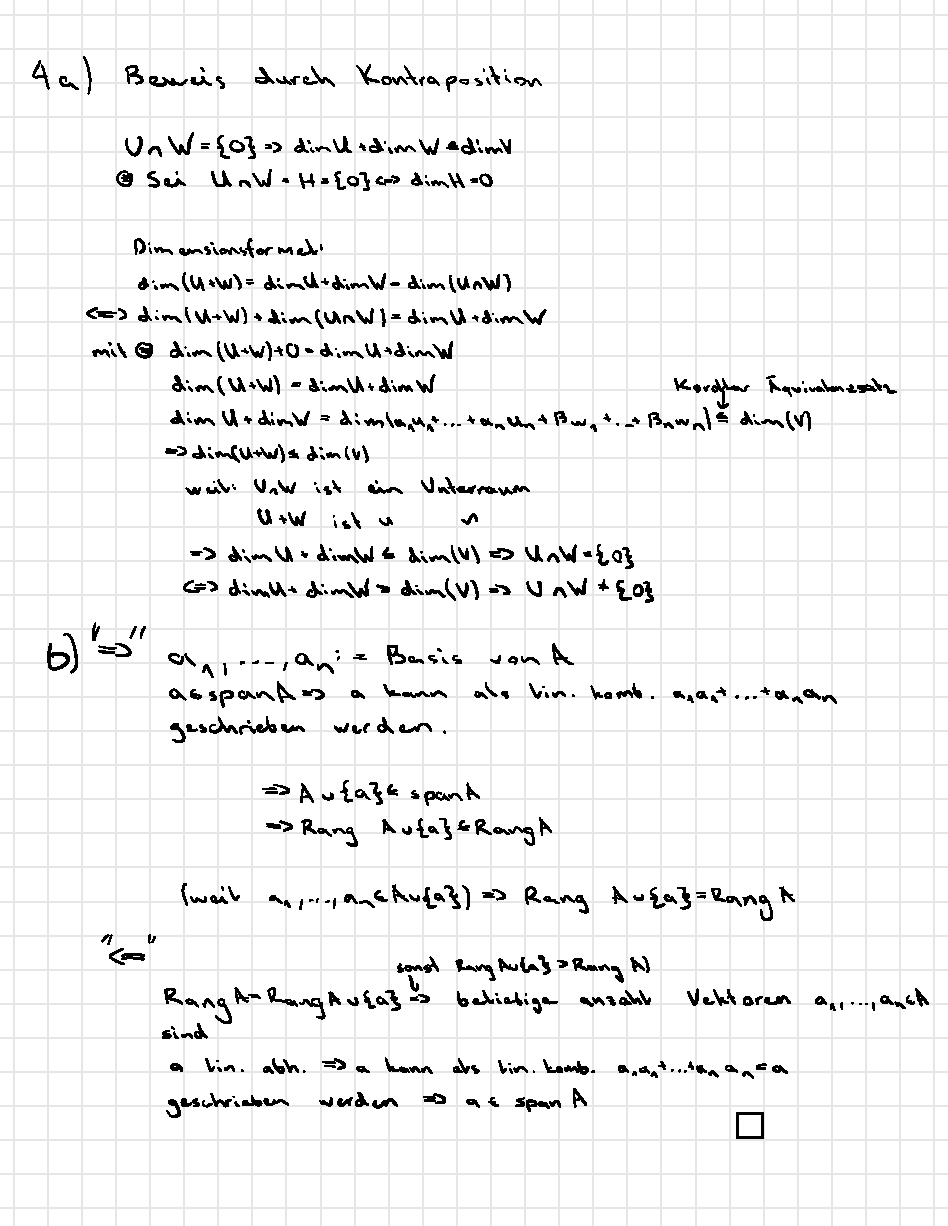
\includegraphics{LinAlg06 Aufg4}
    \end{enumerate}

    \section{Betrachten Sie \newline
    $A=\left(\begin{array}{cccc}1&-1&0&1\\-1&2&1&-1\\0&-2&-3&1\end{array}\right)\in Mat(3,4;\mathbb{R})$
    $b=\left(\begin{array}{c}-1\\2\\-2\end{array}\right)\in \mathbb{R}^3$.
    }
    \begin{enumerate}
        \item[a)]
        \left(\begin{array}{cccccc}1&-1&0&1&|&0\\-1&2&1&-1&|&0\\0&-2&-3&1&|&0\end{array}\right)
        $\rightarrow$\left(\begin{array}{cccccc}1&-1&0&1&|&0\\0&1&1&0&|&0\\0&-2&-3&1&|&0\end{array}\right)
        $\rightarrow$\left(\begin{array}{cccccc}1&0&0&2&|&0\\0&1&0&1&|&0\\0&0&-1&1&|&0\end{array}\right)
        $-x_1 = 2x_4, x_2 = x_4, x_3 = 3_4$
        Basis: $<\left(\begin{array}{c}-2\\-1\\1\\1\end{array}\right)>$
        \item[b)]
        \left(\begin{array}{cccccc}1&-1&0&1&|&-1\\-1&2&1&-1&|&2\\0&-2&-3&1&|&-2\end{array}\right)
        $\rightarrow$\left(\begin{array}{cccccc}1&-1&0&1&|&-1\\0&1&1&0&|&1\\0&-2&-3&1&|&-2\end{array}\right)
        $\rightarrow$\left(\begin{array}{cccccc}1&0&1&1&|&0\\0&1&1&0&|&1\\0&0&-1&1&|&0\end{array}\right)
        \newline
        $\rightarrow$\left(\begin{array}{cccccc}1&0&0&2&|&0\\0&1&0&1&|&1\\0&0&-1&1&|&0\end{array}\right)
        \newline
        $-x_1 = 2x_4, 1-x_2 = x_4, x_3 = 3_4 \Rightarrow(-2,0,1,1)\in L$
        \item[c)]
        \[L=\left\{\left(\begin{array}{c}0\\1\\0\\0\end{array}\right)+\mathbb{R}\left(\begin{array}{c}-2\\-1\\1\\1\end{array}\right)\right\}\]

    \end{enumerate}
\end{document}